\section{Полученные результаты}
\subsection{Тестовые задачи}
Для проверки корректности реализации параллельной версии алгоритма были
произведены расчёты ряда тестовых задач.
\subsubsection{Распространение P-волны}
Для расчёта распространения P-волны в кубе были использованы следующие
безразмерные параметры: 
\begin{itemize}
\item размеры: 50x50x50;
\item $\lambda=70000$;
\item $\nu=10000$;
\item $\rho=1$.
\end{itemize}
На графиках (см. рис.
\ref{pic:p_wave_2}-\ref{pic:p_wave_22}) представленые результаты численного расчёта.
\begin{figure}[htp]
\centering
\includegraphics[width=0.8\textwidth]{png/p-wave-propogation-3d-002.png}
\caption{Распространение P-волны, 2-й временной слой. Слева изображены
напряжения в срезе, перпендикулярном оси x, справа компоненты тензора напряжений
и модуль скорости соответственно.}
\label{pic:p_wave_2}
\end{figure}
\begin{figure}[htp]
\centering
\includegraphics[width=0.8\textwidth]{png/p-wave-propogation-3d-012.png}
\caption{Распространение P-волны, 12-й временной слой. Слева изображены
напряжения в срезе, перпендикулярном оси x, справа компоненты тензора напряжений
и модуль скорости соответственно.}
\label{pic:p_wave_12}
\end{figure}
\begin{figure}[htp]
\centering
\includegraphics[width=0.8\textwidth]{png/p-wave-propogation-3d-022.png}
\caption{Распространение P-волны, 22-й временной слой. Слева изображены
напряжения в срезе, перпендикулярном оси x, справа компоненты тензора напряжений
и модуль скорости соответственно.}
\label{pic:p_wave_22}
\end{figure}
\subsubsection{Распространение S-волны}
Для расчёта распространения S-волны в кубе были использованы следующие
безразмерные параметры: 
\begin{itemize}
\item размеры: 50x50x50;
\item $\lambda=70000$;
\item $\nu=10000$;
\item $\rho=1$.
\end{itemize}
На графиках (см. рис.
\ref{pic:s_wave_2}-\ref{pic:s_wave_22}) представленые результаты численного расчёта.
\begin{figure}[htp]
\centering
\includegraphics[width=\textwidth]{png/s-wave-propogation-3d-002.png}
\caption{Распространение S-волны, 2-й временной слой. Слева изображены
напряжения в срезе, перпендикулярном оси x, справа компоненты тензора напряжений
и модуль скорости соответственно.}
\label{pic:s_wave_2}
\end{figure}
\begin{figure}[htp]
\centering
\includegraphics[width=\textwidth]{png/s-wave-propogation-3d-012.png}
\caption{Распространение S-волны, 12-й временной слой. Слева изображены
напряжения в срезе, перпендикулярном оси x, справа компоненты тензора напряжений
и модуль скорости соответственно.}
\label{pic:s_wave_12}
\end{figure}
\begin{figure}[htp]
\centering
\includegraphics[width=\textwidth]{png/s-wave-propogation-3d-022.png}
\caption{Распространение S-волны, 22-й временной слой. Слева изображены
напряжения в срезе, перпендикулярном оси x, справа компоненты тензора напряжений
и модуль скорости соответственно.}
\label{pic:s_wave_22}
\end{figure}
\subsubsection{Сферический взрыв}
Для проверки корректности расчёта при отражении от границ был произведён расчёт
На графиках (см. рис.
модельной задачи о сферическом взрыве со следующими параметрами:
\begin{itemize}
\item размеры: 50x50x50;
\item $\lambda=70000$;
\item $\nu=10000$;
\item $\rho=1$.
\end{itemize}
На графиках (см. рис. \ref{pic:spherical_25}, \ref{pic:spherical_50}) изображены
результаты расчётов.
\begin{figure}[htp]
\begin{subfigure}[b]{0.5\textwidth}
\centering
\includegraphics[width=\textwidth]{png/v-scalar-0025.png}
\caption{Модули скоростей}
\end{subfigure}
\begin{subfigure}[b]{0.5\textwidth}
\centering
\includegraphics[width=\textwidth]{png/v-vector-0025.png}
\caption{Поле скоростей}
\end{subfigure}
\caption{Расчёт задачи о сферическом врзыве, 25-й временной-слой, волны сжатия и
растяжения. На рисунке слева цветом изображены модули скоростей в трёх взаимно
перпендикулярных плоскостях, а справа -- пое скоростей.}
\label{pic:spherical_25}
\end{figure}
\begin{figure}[htp]
\begin{subfigure}[b]{0.5\textwidth}
\centering
\includegraphics[width=\textwidth]{png/v-scalar-0050.png}
\caption{Модули скоростей}
\end{subfigure}
\begin{subfigure}[b]{0.5\textwidth}
\centering
\includegraphics[width=\textwidth]{png/v-vector-0050.png}
\caption{Поле скоростей.}
\end{subfigure}
\caption{Расчёт задачи о сферическом врзыве, 50-й временной-слой, отражение от
свободной границы. На рисунке слева цветом изображены модули скоростей в трёх взаимно
перпендикулярных плоскостях, а справа -- пое скоростей.}
\label{pic:spherical_50}
\end{figure}
\clearpage
\subsection{Расчёт многослойной преграды}
При расчёте задачи о непробивающем ударе по многослойной преграде использовались
данные из табл. \ref{tbl:subpackage}. В табл. \ref{tbl:subpackage_2} приведены
обезразмеренные величины, использовавшиеся в расчёте.
\begin{table}[h]
\centering
\begin{tabular}{|c|c|c|c|}
\hline
Слой & $\rho$ & $\lambda$ & $\mu$  \\
\hline
Эпоксидная смола & 1.25 & 1440 & 960 \\
Субпакет & 1.25 & 4620 & 3080 \\
\hline
\end{tabular}
\caption{Безразмерные характеристики субпакетов.}
\label{tbl:subpackage_2}
\end{table}
\itodo{Параметры удара?}
На графиках (см. рис. \ref{pic:multilayer_init}-\ref{pic:multilayer_Rayleigh_2})
изображены результаты численного расчёта задачи.
\begin{figure}[htp]
\centering
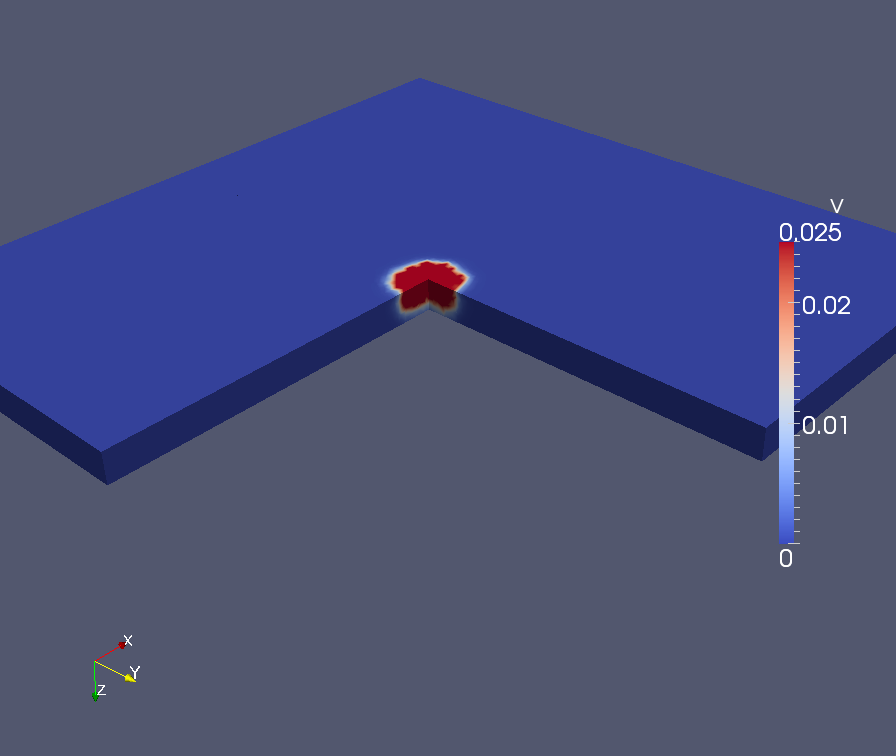
\includegraphics[width=\textwidth]{png/v-0001.png}
\caption{Начальное возмущение. На рисунке цветом изображены модули скоростей в
двух взаимно перпендикулярных срезах.}
\label{pic:multilayer_init}
\end{figure}
\begin{figure}[htp]
\centering
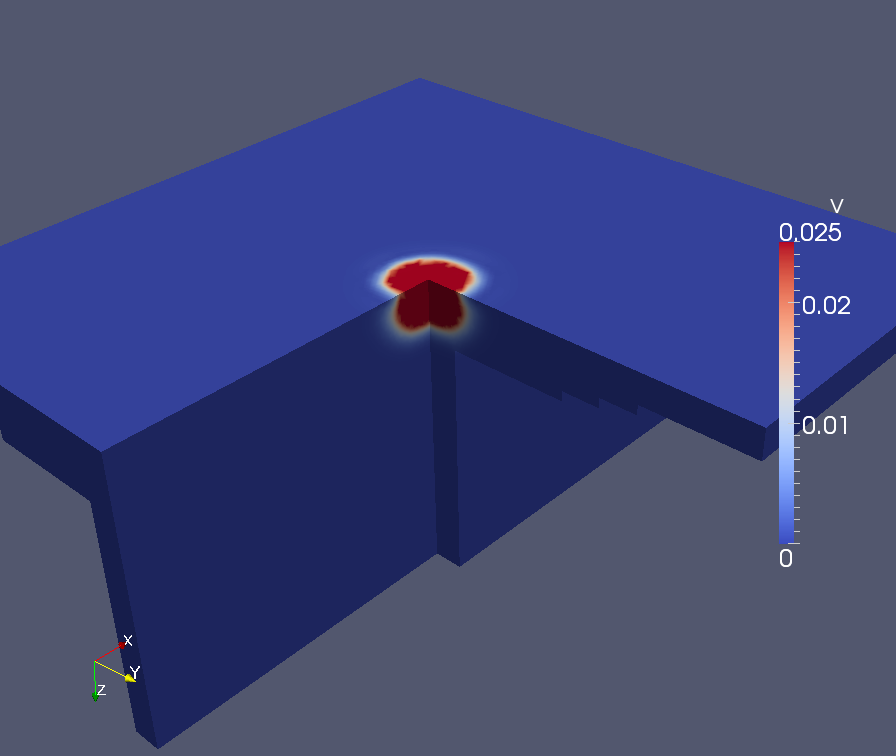
\includegraphics[width=\textwidth]{png/v-0003.png}
\caption{Отражение от первой границы. На рисунке цветом изображены модули скоростей в
двух взаимно перпендикулярных срезах.}
\label{pic:multilayer_b1}
\end{figure}
\begin{figure}[htp]
\centering
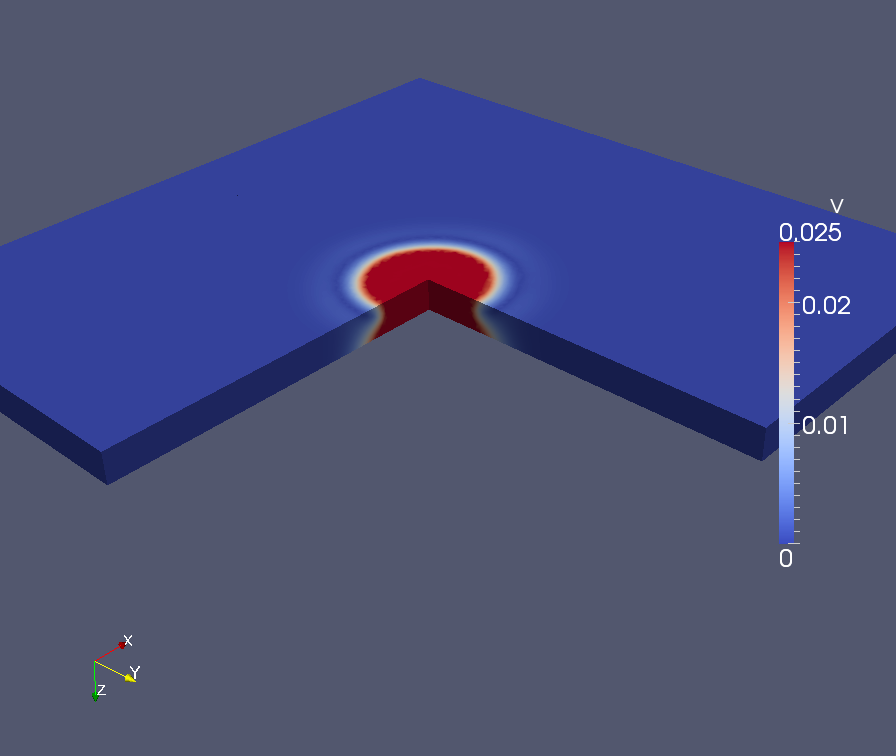
\includegraphics[width=\textwidth]{png/v-0007.png}
\caption{Отражение от второй границы. На рисунке цветом изображены модули скоростей в
двух взаимно перпендикулярных срезах.}
\label{pic:multilayer_b2}
\end{figure}
\begin{figure}[htp]
\centering
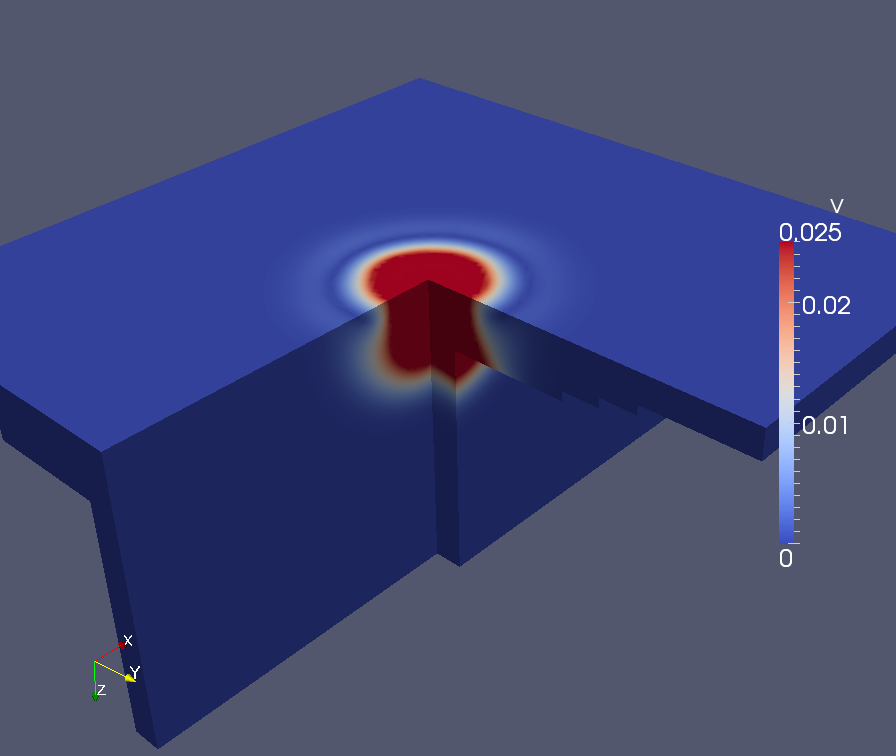
\includegraphics[width=\textwidth]{png/v-0009.png}
\caption{Отражение от третьей границы. На рисунке цветом изображены модули скоростей в
двух взаимно перпендикулярных срезах.}
\label{pic:multilayer_b3}
\end{figure}
\begin{figure}[htp]
\centering
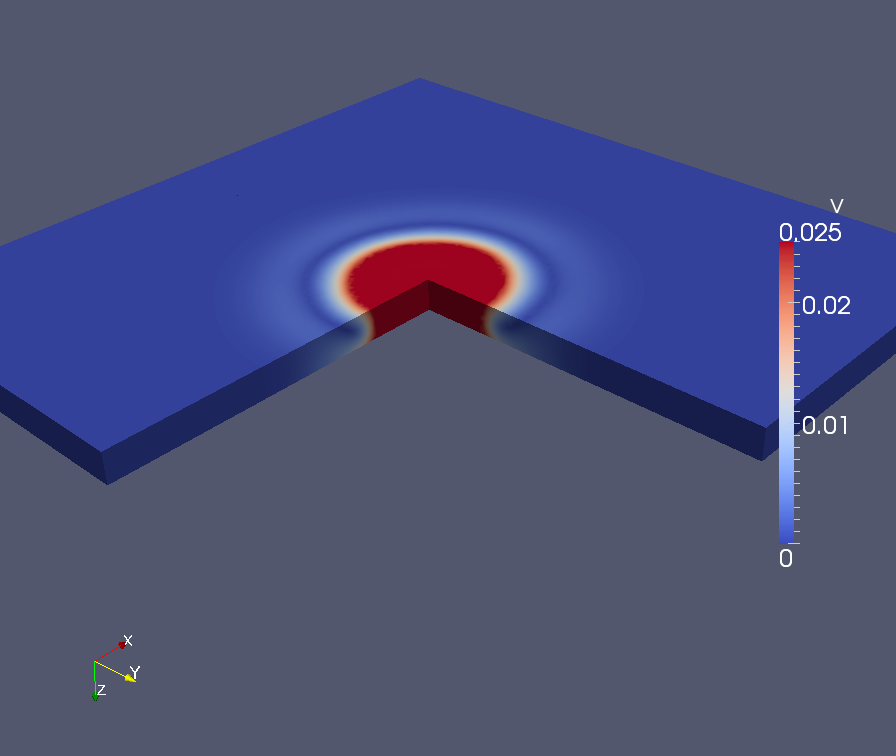
\includegraphics[width=\textwidth]{png/v-0013.png}
\caption{Формирование волны Рэлея. На рисунке цветом изображены модули скоростей
в срезе, перпендикулярном оси x, а стрелками обозначены поля скоростей.}
\label{pic:multilayer_b3}
\end{figure}
\begin{figure}[htp]
\centering
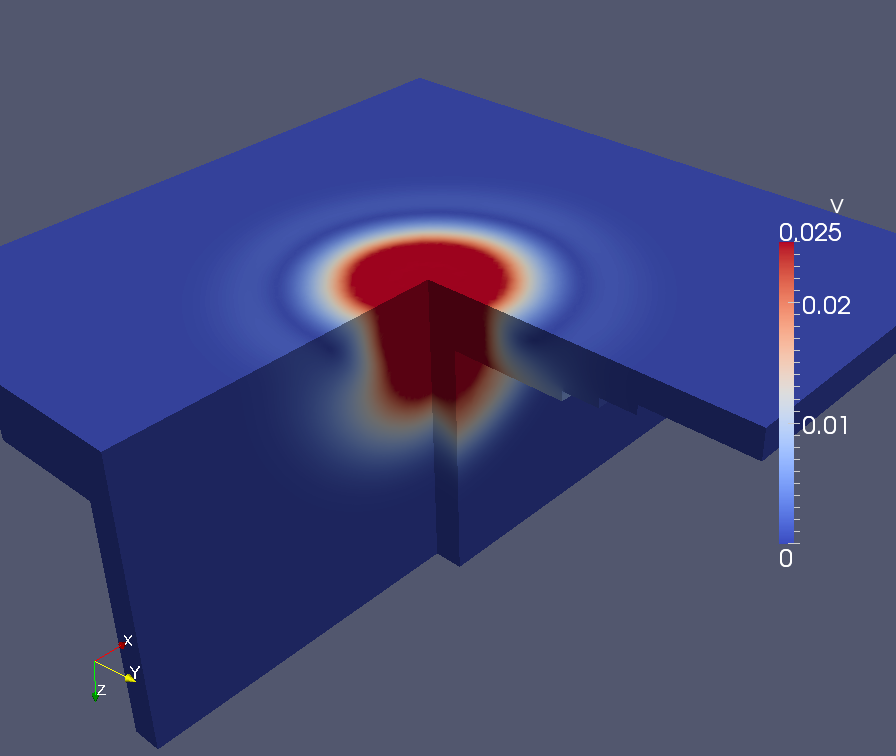
\includegraphics[width=\textwidth]{png/v-0016.png}
\caption{Распространение волны Рэлея. На рисунке цветом изображены модули скоростей
в срезе, перпендикулярном оси x, а стрелками обозначены поля скоростей.}
\label{pic:multilayer_Rayleigh_2}
\end{figure}
